%!TEX root = ../Report.tex
%************************************************

% Detail design

\chapter{Results}
This chapter outlines the results, including the design of the user interface, functionality of the application and a short summary of the results of the incorporated algorithms.
The majority of the results have already been covered in part \ref{part:algo}, however a discussion is provided.

\section{User interface}

\begin{figure}
\centerline{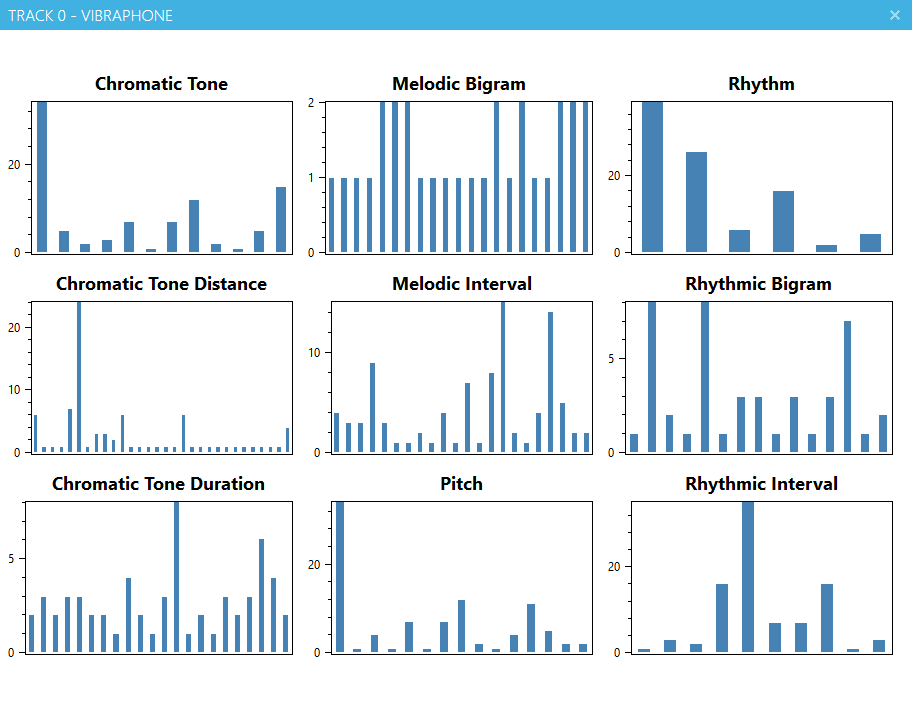
\includegraphics[width=400px]{../images/res_ui_metrics_harry_t0.png}}
\caption{Frequency metrics for the first track Harry Potter Opening Theme Song}
\label{ims:metricsharryt0}
\end{figure}

Figure \ref{ims:metricsharryt0} shows the frequency metrics for the first track of the Harry Potter opening theme song.

\begin{figure}
\centerline{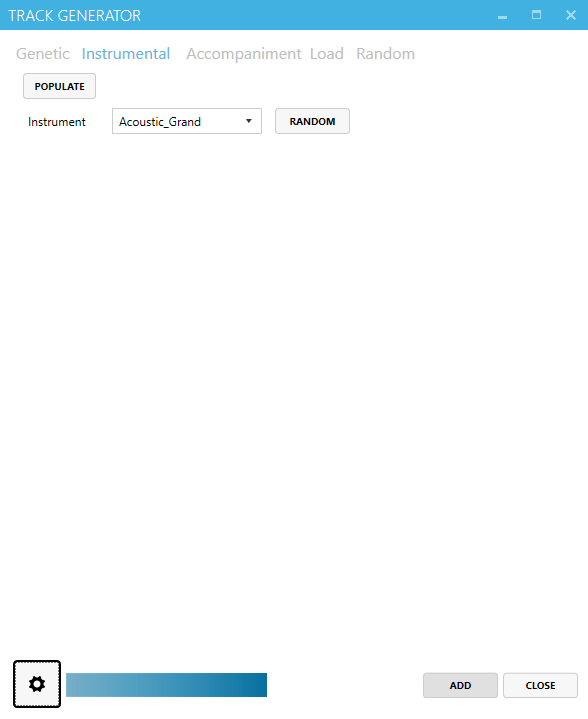
\includegraphics[width=400px]{../images/res_ui_track_generator_instr.png}}
\caption{Window of instrumental tab in track generator}
\label{ims:uitrackgeninstr}
\end{figure}

Figure \ref{ims:uitrackgeninstr} indicates the window of the track generator with the instrumental tab selected. Here a Markov Chains generates a instrumental melody for the Acoustic Grand instrument.


\chapter{Conclusion}
The aim of this project was to design an application that is able to compose melodies in a certain musical style using machine learning algorithms. A brief survey was done on existing attempts to compose melodies using machine learning techniques.
\\

Evolutionary algorithms are versatile and are well suited to the the task of musical composition. The task of designing a good fitness function for a genetic algorithm is rather formidable.
Musical composition is a emotional human process and is subjective in nature. This makes formalization of what constitutes a good melody difficult. 
An attempt was made by using the \ac{NCD} to rate the fitness of melodies, however the results were not satisfactory.
Decent results were obtained by using frequency metrics in conjuction with a similarity measure. This approach provides high fitness to individuals which have similar statistical properties to the target piece. The problem with the approach is that a high statistical similarity may be achieved but this does not necesarily imply that a individual will be perceived as pleasant or good.
\\

A different approach was taken thereafter, other than relying on statistical properties and requiring a function to quantify the pleasantness of a melody. A probalistic approach was taken to predict the pattern of melodies. By employing the Markov property - the probability distribution of future states depend only upon the present states simplifications can be made and Markov Models can be designed. The simplest Markov Model, the Markov Chain produced pleasant results. A third order Markov Chain, where the next note is determined by the preceeding 3 notes produced pleasant results without sacrificing too much novelty and avoiding too much similarity. By employing another Markov Model, attempt was made to produce an accompaniment for a melody, by calculating the probilities for an accompaniment note by the preceeding 2 notes in the melody track. This Markov Model also yielded satisfactory results however more work is required on timing and synchronization.
Overall these probalistic models yield good results, however the melodies produce lack an overarching theme and structure. Furthermore since Markov Models a input dataset and calculate the transmission and emission probabilities based on the input data the novelty and composition value are low. These models produce pleasant results but are not creative or original.
\\

Further works is needed to develop an algorithm that is able to compose melodies that have an overarching theme or structure.  Further work can be done using recurrent neural networks in a variety of topologies or using a custom Hidden Markov Models. These techniques were used in a simplistic way to generate the accompaniment to a melody with acceptable results.
\\

The results of most the algorithms could be improved by incorporating domain knowledge into the system. Musical knowledge could constrain the algorithm to produce more acceptable results. A hybrid system that incorporates expert knowledge may reduce the number of unpleasant patterns produced and improve note transitions and so forth.
\\

The application used a number of simplifications. A major simplification was that only monophonic melodies were considered, no chords. A more advanced system can be designed that applies the investigated algorithms to chords as well. Further algorithms could be used for harmonization.
\\

The application conforms to the specifications and is able to satisfactorily produce melodies in Classical, Jazz, Drum and Video Games styles using Markov Chains, Neural Networks and Genetic Algorithms.

\chapter{Future Work}